% LaTeX figure snippets generated by the plot agent. All underlying values
% trace directly to inputs/experimental_log.md. Categorical panels encode
% qualitative statements (detected / reduced / absent, present / partial /
% absent) rather than fabricating numeric measurements.

\begin{figure}[htbp]
\centering
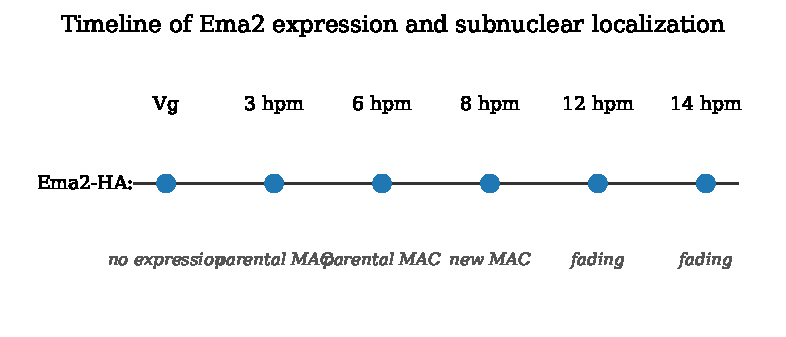
\includegraphics[width=0.85\textwidth]{figures/fig1_ema2_timeline.pdf}
\caption{Timeline of Ema2 expression and subnuclear localization during
conjugation. Ema2-HA is undetectable in vegetatively growing cells (Vg),
first appears in the parental MAC at 3 and 6~hpm, relocates to the new MAC
by 8~hpm, and fades by 12 and 14~hpm. Schematic compiled from the
experimental log narrative of Figures~1A--B.}
\label{fig:timeline}
\end{figure}

\begin{figure}[htbp]
\centering
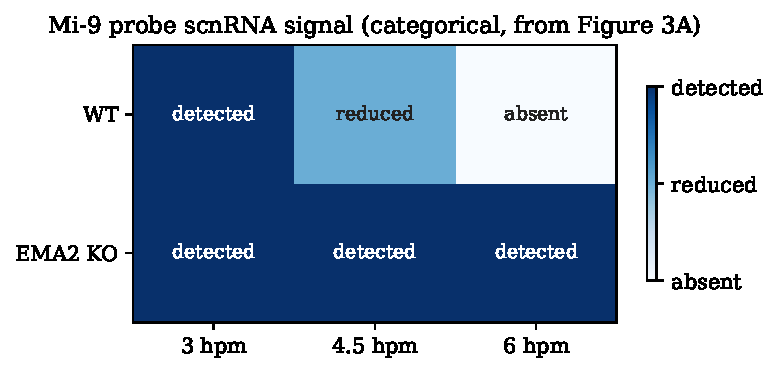
\includegraphics[width=0.75\textwidth]{figures/fig2_tdsd_schematic.pdf}
\caption{Categorical representation of Mi-9 probe scnRNA signal across
conjugation time points for wild-type and EMA2 KO cells (from the narrative
of Figure~3A). Wild-type cells show detected, reduced and absent signal at
3, 4.5 and 6~hpm respectively, consistent with target-directed small RNA
degradation. EMA2 KO cells retain detectable signal at all three time points.}
\label{fig:tdsd}
\end{figure}

\begin{figure}[htbp]
\centering
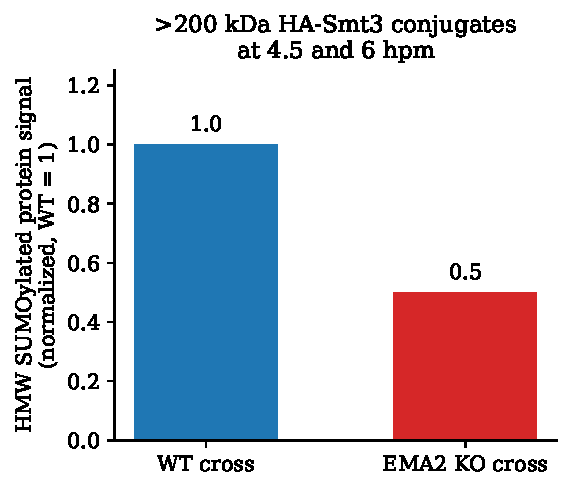
\includegraphics[width=0.55\textwidth]{figures/fig3_sumo_bar.pdf}
\caption{Quantification of high molecular weight ($>\!200$~kDa) HA-Smt3
conjugates detected in the WT cross and the EMA2 KO cross. Signals from the
WT cross were normalized to 1; the EMA2 KO cross shows approximately 50\% of
the wild-type level, as stated in the extraction of Figure~4C.}
\label{fig:sumo}
\end{figure}

\begin{figure}[htbp]
\centering
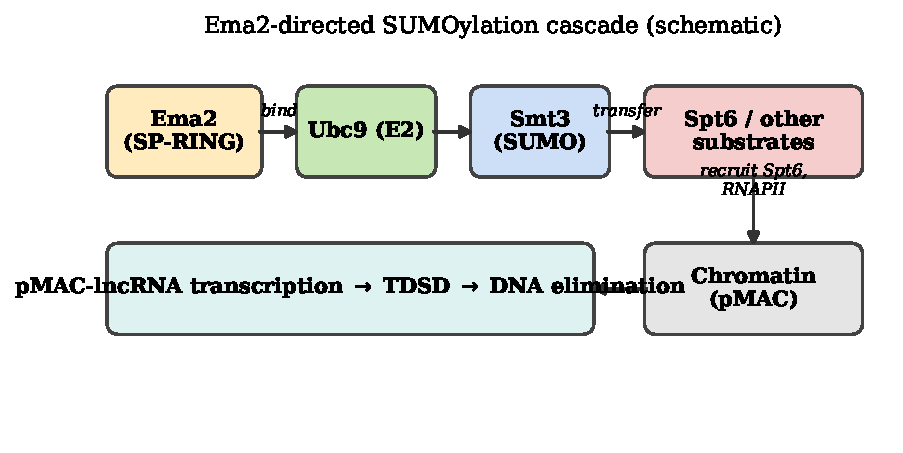
\includegraphics[width=0.85\textwidth]{figures/fig4_pathway_schematic.pdf}
\caption{Schematic of the Ema2-directed SUMOylation cascade. Ema2 (SP-RING)
binds the SUMO E2 Ubc9, which transfers Smt3 onto Spt6 and additional
substrates; SUMOylated Spt6 is retained on parental MAC chromatin to permit
pMAC-lncRNA transcription, which in turn drives TDSD and programmed DNA
elimination.}
\label{fig:pathway}
\end{figure}

\begin{figure}[htbp]
\centering
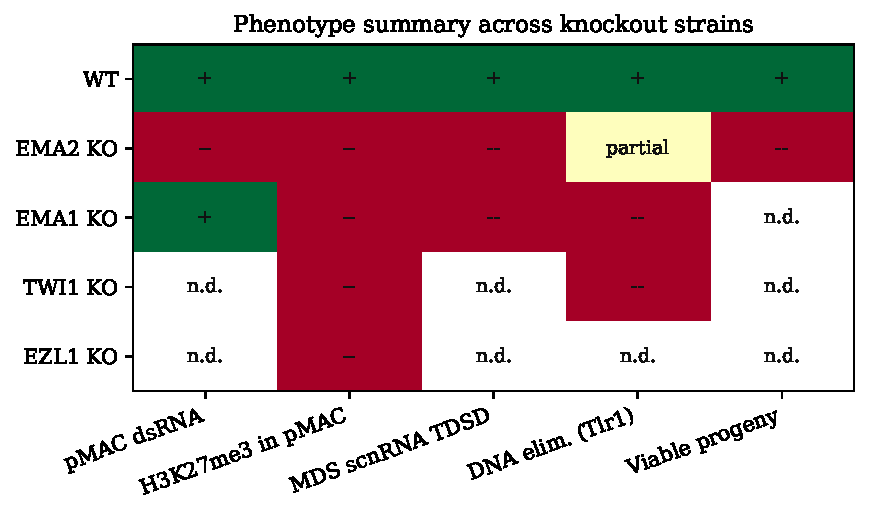
\includegraphics[width=0.85\textwidth]{figures/fig5_phenotype_matrix.pdf}
\caption{Phenotype summary across knockout strains compiled from the
experimental log. A plus sign denotes the feature is present or complete,
minus denotes absent or defective, ``partial'' denotes an intermediate
phenotype (e.g., the DNA elimination defect of EMA2 KO relative to TWI1~KO),
and ``n.d.'' denotes features that are not explicitly measured for that
strain in the extraction.}
\label{fig:phenotypes}
\end{figure}

\begin{figure}[htbp]
\centering
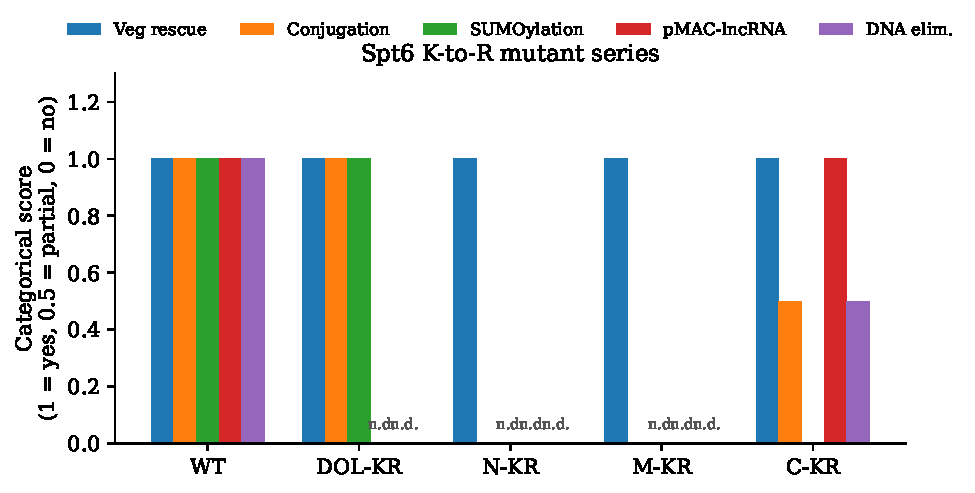
\includegraphics[width=0.9\textwidth]{figures/fig6_spt6_mutants.pdf}
\caption{Summary of the Spt6 K-to-R mutant series. All constructs rescue
vegetative SPT6 KO lethality. HA-SPT6-N-KR and HA-SPT6-M-KR show severe
defects in meiotic progression and mating initiation, respectively; HA-SPT6
-DOL-KR is SUMOylated like wild-type Spt6, whereas HA-SPT6-C-KR shows no
detectable SUMOylation yet still supports chromatin association of Spt6
and RNAPII, parental-MAC dsRNA accumulation, and only a mild DNA elimination
defect. Hatched bars with ``n.d.'' indicate features not examined for that
mutant in the extraction.}
\label{fig:spt6mutants}
\end{figure}
